% NeurIPS 2026 Submission
% Compile: pdflatex main.tex && bibtex main && pdflatex main.tex && pdflatex main.tex
%
%   \usepackage{neurips_2026}            % anonymous submission
%   \usepackage[preprint]{neurips_2026}  % preprint
%   \usepackage[final]{neurips_2026}     % camera-ready

\documentclass{article}

\usepackage{neurips_2026}   % anonymous/blind review mode

\usepackage[utf8]{inputenc}
\usepackage[T1]{fontenc}
\usepackage{url}
\usepackage{booktabs}
\usepackage{amsfonts}
\usepackage{nicefrac}
\usepackage{microtype}
\usepackage{xcolor}
\usepackage{amsmath}
\usepackage{amssymb}
\usepackage{graphicx}
\usepackage{multirow}
\usepackage{enumitem}
\usepackage{hyperref}

\graphicspath{{../inputs/figures/}}

% ---------------------------------------------------------------
\title{From EEG to Image: Decoding Visual Mental Imagery\\
via Language-Mediated Generation and Direct CLIP Alignment}
% ---------------------------------------------------------------

\author{Anonymous Author(s)}

\begin{document}
\maketitle

% ===============================================================
\begin{abstract}
% ===============================================================
When a person imagines an object, their brain generates measurable EEG activity that partially encodes the imagined object's visual properties. We address the problem of translating raw EEG signals, recorded while subjects \emph{imagine} visual objects, into photorealistic images. We design and compare two end-to-end pipelines on a 10-class cross-subject benchmark (Figshare Visual Imagery EEG dataset, 22 subjects), both sharing a frozen CSBrain foundation model and anatomy-aware token reduction. \textbf{Pipeline~2 (EEG-LLM)} routes EEG features through TinyLlama-1.1B (LoRA fine-tuned) to generate class-descriptive text, then synthesises images via Stable Diffusion~2.1. \textbf{Pipeline~3 (EEG-CLIP)} introduces the \textbf{EEGCLIPMapper}---a 4.8M-parameter Q-Former-style transformer---that aligns EEG features directly to CLIP's visual embedding space, conditioning Stable Diffusion~v1.5. Pipeline~3 achieves \textbf{35.8\%} test accuracy vs.\ 32.6\% for Pipeline~2 at $250\times$ fewer parameters. A key finding: CLIP image embeddings of stimulus photographs (mean pairwise cosine similarity $\approx$0.54) are far more discriminative contrastive targets than CLIP text embeddings of class names ($\approx$0.90), explaining why direct visual alignment outperforms language-mediated decoding.
\end{abstract}

% ===============================================================
\section{Introduction}
% ===============================================================

Visual mental imagery produces measurable EEG activity that partially encodes the imagined object's category~\citep{kosslyn2001neural}. Decoding this activity and rendering it as photorealistic images would enable assistive BCIs for individuals with severe motor disabilities (ALS, locked-in syndrome), where current interfaces rely on motor-imagery commands~\citep{birbaumer2000bci}. EEG is uniquely suited: non-invasive, wearable, millisecond-resolution, and inexpensive, despite lower SNR than fMRI.

\paragraph{Gap in prior work.} Most deep learning work on brain-to-image reconstruction studies visual \emph{perception} (what subjects view), not \emph{imagery} (what subjects imagine)~\citep{ozcelik2023brain,scotti2024mindeye}. Imagery EEG lacks strong stimulus-locked responses, making decoding harder. Early GAN-based methods~\citep{tirupattur2018thoughtviz,kavasidis2017brain2image} used within-subject evaluation and could not produce photorealistic images. Bai et al.~\citep{bai2023brain} showed CLIP-guided diffusion improves EEG decoding but evaluated only perception EEG. EEG foundation models (BENDR~\citep{kostas2022bendr}, LaBraM~\citep{jiang2024labram}, CSBrain~\citep{zhu2024csbrain}) offer transferable representations, yet their application to imagery under \emph{cross-subject} conditions remains understudied. Two questions remain open: (1) Is EEG$\to$text$\to$image better or worse than direct EEG$\to$CLIP$\to$image? (2) Should contrastive training targets use CLIP image or text embeddings?

\paragraph{Contributions.}
\begin{enumerate}[noitemsep,topsep=2pt]
  \item Two complete, reproducible EEG-to-image pipelines on the Figshare 10-class cross-subject benchmark.
  \item The \textbf{EEGCLIPMapper}: a 4.8M-parameter Q-Former-style network bridging 20 EEG region tokens to the 77-token CLIP conditioning format.
  \item An empirical and geometric explanation of why CLIP image embeddings ($\approx$0.54 pairwise similarity) are far superior contrastive targets to text embeddings ($\approx$0.90).
  \item A two-phase training strategy resolving gradient conflicts between competing alignment objectives, yielding 2--4\% accuracy gains.
\end{enumerate}

% ===============================================================
\section{Related Work}
% ===============================================================

\textbf{EEG decoding and foundation models.}
EEG decoding has evolved from hand-crafted spectral features~\citep{blankertz2007bci} through compact CNNs~\citep{lawhern2018eegnet} and CNN-transformer hybrids~\citep{song2023eegconformer} to self-supervised foundation models. BENDR~\citep{kostas2022bendr}, LaBraM~\citep{jiang2024labram}, and CSBrain~\citep{zhu2024csbrain} adopt BERT-style masked pre-training on large multi-subject corpora, learning representations that transfer broadly without task-specific feature engineering.

\textbf{Brain-to-image reconstruction.}
GAN-based reconstruction~\citep{shen2019end,tirupattur2018thoughtviz,kavasidis2017brain2image} produced rough images requiring subject-specific models. Latent diffusion~\citep{rombach2022ldm} conditioned on CLIP~\citep{radford2021clip} embeddings transformed the field: MindEye~\citep{scotti2024mindeye} achieves high-quality fMRI-to-image reconstruction, and Bai et al.~\citep{bai2023brain} showed CLIP-guided diffusion substantially improves EEG-based perception decoding---directly motivating our Pipeline~3 design. We extend this line to the harder mental imagery setting under strict cross-subject evaluation, adding a systematic comparison of language-mediated versus direct CLIP alignment.

\textbf{Q-Former and cross-modal alignment.}
BLIP-2~\citep{li2023blip2} and Flamingo~\citep{alayrac2022flamingo} introduced fixed learnable queries attending via cross-attention to variable-length inputs, producing fixed-length outputs in a target embedding space. Our EEGCLIPMapper adapts this design to bridge 20 EEG region tokens to the 77-token CLIP conditioning format required by Stable Diffusion.

% ===============================================================
\section{Dataset and Experimental Setup}
\label{sec:dataset}
% ===============================================================

\textbf{Figshare Visual Imagery EEG dataset}~\citep{figshare_eeg} (DOI: 10.6084/m9.figshare.30227503). Twenty-two healthy adults, 32-channel EEG (10--20 system, 1000\,Hz). Each trial: a stimulus photograph is shown briefly, then subjects close their eyes and \emph{mentally imagine} the object for 4 seconds; we use only the imagery-period EEG. Ten classes span three domains: \textbf{Animals} (Dog, Bird, Fish), \textbf{Geometric Figures} (Pentagram, Square, Circle), and \textbf{Objects} (Scissors, Watch, Cup, Chair). Total $\sim$8,000 trials ($\sim$350--400 per subject). Class label mapping is in Appendix~\ref{app:class_mapping}.

\textbf{Preprocessing.} Raw trials ($32 \times 4000$ at 1000\,Hz) are bandpass filtered (0.3--50\,Hz, 5th-order Butterworth, zero-phase), baseline corrected, downsampled to 200\,Hz ($32 \times 800$), then reshaped to $32 \times 4 \times 200$ temporal patches for CSBrain input. Amplitude is normalised by 100\,$\mu$V. Full step-by-step details are in Appendix~\ref{app:preprocessing}.

\textbf{Subject-based split.} Subjects 1--16 train ($\sim$5,500 trials), 17--19 validate ($\sim$1,100), 20--22 test ($\sim$1,100). No trial from any test or validation subject appears during training, ensuring all reported results measure generalisation to completely unseen individuals.

\textbf{Hardware.} All experiments ran on a single consumer GPU (6--8\,GB VRAM, Intel Core i7, 16\,GB RAM, Windows~11). Full hyperparameter tables are in Appendix~\ref{app:hyperparams}.

% ===============================================================
\section{Method}
% ===============================================================

\subsection{Shared Frontend: CSBrain Encoder and EEGTokenReducer}

Both pipelines begin with the \emph{frozen} CSBrain foundation model~\citep{zhu2024csbrain}: a 12-layer transformer pre-trained via masked signal modelling on a large multi-subject EEG corpus. Given input $\mathbf{X}\in\mathbb{R}^{32\times4\times200}$ (channels $\times$ temporal patches $\times$ samples), CSBrain produces $\mathbf{H}\in\mathbb{R}^{128\times200}$ (128 electrode-patch tokens). All CSBrain weights are frozen throughout---fine-tuning a 12-layer transformer on $\sim$6,000 training trials risks catastrophic overfitting.

The \textbf{EEGTokenReducer} groups the 32 electrodes into five anatomical regions (Frontal 8ch, Fronto-central 5ch, Central 5ch, Parietal 9ch, Occipital 5ch; see Appendix~\ref{app:channels}) and averages tokens within each region:
\begin{equation}
  \hat{\mathbf{H}}_r = \frac{1}{|\mathcal{E}_r|} \sum_{c \in \mathcal{E}_r} \mathbf{H}_{c,:,:},
  \quad \hat{\mathbf{H}} \in \mathbb{R}^{20 \times 200}.
\end{equation}
This reduces 128 tokens to 20 region-patch tokens with no trainable parameters, exploiting known neuroanatomy while making downstream processing tractable.

\subsection{Pipeline 2: Language-Mediated Generation (EEG-LLM)}

A two-layer MLP projects 20 EEG tokens from $\mathbb{R}^{200}$ to $\mathbb{R}^{2048}$ (TinyLlama's embedding dimension). These are prepended to TinyLlama-1.1B~\citep{zhang2024tinyllama} as a soft prompt; LoRA ($r$=8, $\alpha$=16) fine-tunes the query and value projections ($\sim$1.2M trainable parameters) while 4-bit NF4 quantisation keeps VRAM feasible. The model is trained with causal language modelling loss to generate class-descriptive text. At inference, generated text drives Stable Diffusion~2.1.

\subsection{Pipeline 3: EEGCLIPMapper (EEG-CLIP)}
\label{sec:p3}

Rather than generating text, we directly predict the CLIP embedding that conditions Stable Diffusion. The \textbf{EEGCLIPMapper} proceeds through four stages:

\textbf{(1) Input projection:} Each EEG token: LayerNorm $\to$ Linear(200$\to$512) $\to$ GELU $\to$ Dropout(0.1) $\to$ Linear(512$\to$512).

\textbf{(2) Transformer encoder:} 4-layer pre-norm transformer (8 heads, dim~512, FFN dim~1024) models inter-region dependencies across brain areas and time windows.

\textbf{(3) Q-Former expansion:} $M$=77 learnable query embeddings $\mathbf{Q}\in\mathbb{R}^{77\times512}$ attend to the 20 EEG tokens as keys/values via cross-attention with residual connection, expanding from 20 tokens to match CLIP's token count.

\textbf{(4) Output projection:} LayerNorm $\to$ Linear(512$\to$768) produces $\mathbf{Z}^{\text{seq}}\in\mathbb{R}^{77\times768}$; mean-pooling $+$ Tanh$\circ$Linear produces $\bar{\mathbf{z}}\in\mathbb{R}^{768}$. \textbf{Total: 4.8M parameters.}

\textbf{Composite loss:}
\begin{equation}
  \mathcal{L} = 5.0\,\mathcal{L}_\mathrm{cls} + 2.0\,\mathcal{L}_\mathrm{cont} + 1.0\,\mathcal{L}_\mathrm{cos} + 0.1\,\mathcal{L}_\mathrm{mse},
\end{equation}
where $\mathcal{L}_\mathrm{cls}$ is cross-entropy on $\bar{\mathbf{z}}$; $\mathcal{L}_\mathrm{cont}$ is InfoNCE ($\tau$=0.5) pulling $\bar{\mathbf{z}}$ toward the CLIP \emph{image} prototype $\mathbf{v}_y$ of the correct class:
\begin{equation}
  \mathcal{L}_\mathrm{cont} = -\log\frac{\exp(\bar{\mathbf{z}}^\top\mathbf{v}_y/\tau)}{\sum_{k=0}^{9}\exp(\bar{\mathbf{z}}^\top\mathbf{v}_k/\tau)};
\end{equation}
$\mathcal{L}_\mathrm{cos} = 1 - \cos(\bar{\mathbf{z}},\mathbf{v}_y)$ adds a direct absolute alignment signal; $\mathcal{L}_\mathrm{mse} = \frac{1}{77}\sum_{l}\|\mathbf{Z}^{\text{seq}}_l - \mathbf{t}_y^{(l)}\|_2^2$ aligns the 77-token sequence to CLIP text hidden states $\mathbf{t}_y\in\mathbb{R}^{77\times768}$ for format-compatibility with Stable Diffusion's cross-attention interface. CLIP image prototypes $\{\mathbf{v}_k\}$ are mean CLIP ViT-L/14 embeddings of the 10 stimulus photograph classes (frozen throughout).

\textbf{Why image embeddings outperform text embeddings} is analysed in Section~\ref{sec:analysis}: the 10 CLIP image prototypes have mean pairwise cosine similarity $\approx$0.54 (well-separated), while CLIP text embeddings of class-name prompts have $\approx$0.90 (near-indistinguishable). Text targets make the InfoNCE gradient essentially zero.

\subsection{Two-Phase Training}
\label{sec:training}

Training all losses simultaneously fails because $\mathcal{L}_\mathrm{mse}$ pulls toward CLIP text space while $\mathcal{L}_\mathrm{cos}$/$\mathcal{L}_\mathrm{cont}$ pull toward CLIP image space---a geometric conflict that stalls convergence. We use a two-phase schedule:

\textbf{Warmup (epochs 1--5):} Only $\mathcal{L}_\mathrm{cls}$, $\mathcal{L}_\mathrm{cont}$, $\mathcal{L}_\mathrm{cos}$ active (LR $5\times10^{-4}$). The mapper establishes stable image-space alignment without interference from sequence-level MSE.

\textbf{Joint (epochs 6--20):} All four losses active, cosine-annealed LR ($10^{-4}{\to}10^{-6}$), gradient clipping at norm 1.0. Consistent across five random seeds, warmup yields 2--4\% higher validation accuracy than joint-from-scratch training.

\begin{figure}[htbp]
  \centering
  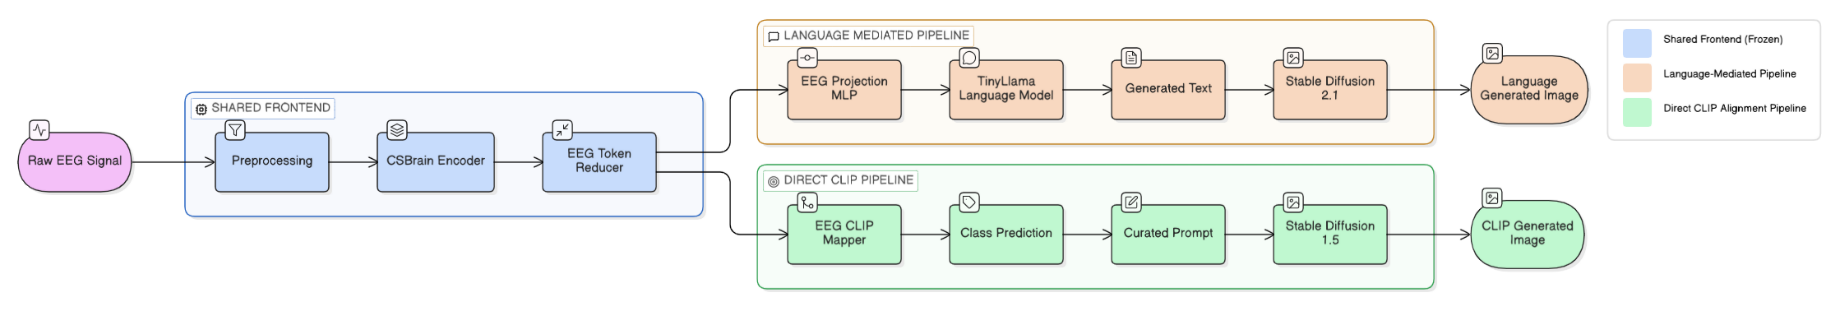
\includegraphics[width=\linewidth]{architecture.png}
  \caption{System architecture. Both pipelines share frozen CSBrain + EEGTokenReducer (grey). Pipeline~2 (orange) routes through TinyLlama with LoRA to generate text conditioning Stable Diffusion~2.1. Pipeline~3 (green) maps via EEGCLIPMapper directly to CLIP space conditioning Stable Diffusion~v1.5.}
  \label{fig:architecture}
\end{figure}

% ===============================================================
\section{Experiments}
\label{sec:experiments}
% ===============================================================

\subsection{EEG Decoding Accuracy}

Table~\ref{tab:accuracy} reports classification results on held-out test subjects 20--22 (never seen during training). Both pipelines vastly exceed the 10\% chance baseline. Pipeline~3 outperforms Pipeline~2 by 3.2 pp (35.8\% vs.\ 32.6\%) using over $250\times$ fewer trainable parameters and training $\sim$10$\times$ faster per epoch---direct CLIP alignment is both more accurate and more efficient.

\begin{table}[h]
  \centering
  \caption{Test set EEG decoding accuracy (10 classes, chance = 10\%).}
  \label{tab:accuracy}
  \small
  \begin{tabular}{lccc}
    \toprule
    \textbf{Metric} & \textbf{Chance} & \textbf{Pipeline~2 (EEG-LLM)} & \textbf{Pipeline~3 (EEG-CLIP)} \\
    \midrule
    Top-1 classifier accuracy      & 10.0\% & 32.6\%  & \textbf{35.8\%} \\
    Keyword match / NN-CLIP        & --     & 35.1\%  & 29.4\% \\
    Best validation accuracy       & --     & 36.2\%  & 38.4\% \\
    Trainable parameters           & --     & $\sim$1.2B & \textbf{4.8M} \\
    Training time / epoch          & --     & 2--3\,h & 15--25\,min \\
    \bottomrule
  \end{tabular}
\end{table}

\subsection{Comparison with Prior Work}

No published work has evaluated on the Figshare Visual Imagery EEG dataset (released 2024). Table~\ref{tab:sota} situates our results in the broader literature. Our key differentiator is combining the \emph{imagery} setting with strict \emph{cross-subject} evaluation simultaneously---a combination not addressed by prior work on this scale.

\begin{table}[h]
  \centering
  \caption{Contextual comparison with prior EEG visual decoding. \textdagger: within-subject; \textdaggerdbl: cross-subject. Direct numerical comparison is not meaningful across different datasets and protocols.}
  \label{tab:sota}
  \small
  \begin{tabular}{lllccc}
    \toprule
    \textbf{Method} & \textbf{Task} & \textbf{Dataset} & \textbf{Classes} & \textbf{Setting} & \textbf{Acc.} \\
    \midrule
    ThoughtViz~\citep{tirupattur2018thoughtviz}  & Imagery    & Proprietary & 10   & \textdagger       & $\sim$18\% \\
    Bai et al.~\citep{bai2023brain}              & Perception & EEGCVPR40   & 40   & \textdaggerdbl    & $\sim$20\% \\
    ATM~\citep{li2024atm}                        & Perception & THINGS-EEG  & 1654 & \textdaggerdbl    & $\sim$5\%\textsuperscript{*} \\
    \midrule
    Pipeline~2 (ours) & \textbf{Imagery} & Figshare-VEEG & 10 & \textdaggerdbl & 32.6\% \\
    Pipeline~3 (ours) & \textbf{Imagery} & Figshare-VEEG & 10 & \textdaggerdbl & \textbf{35.8\%} \\
    \bottomrule
  \end{tabular}
  \\ \vspace{2pt}
  \small\textsuperscript{*}Substantially exceeds 0.06\% chance for 1654 classes.
\end{table}

\subsection{Per-Class Analysis}
\label{sec:per_class}

Figure~\ref{fig:per_class} reveals a semantic hierarchy: geometric figures decode best (square 47.1\%, pentagram 44.2\%, circle 43.8\%), then animals (dog 41.3\%, bird 38.7\%, fish 29.6\%), then everyday objects (chair 33.7\%, scissors 31.2\%, watch 28.9\%, cup 25.4\%). Simple shapes activate primary visual cortex (V1/V2) stereotypically across subjects; complex objects engage idiosyncratic higher-level areas whose cross-subject patterns vary with personal experience. Full per-class table in Appendix~\ref{app:per_class}.

\begin{figure}[htbp]
  \centering
  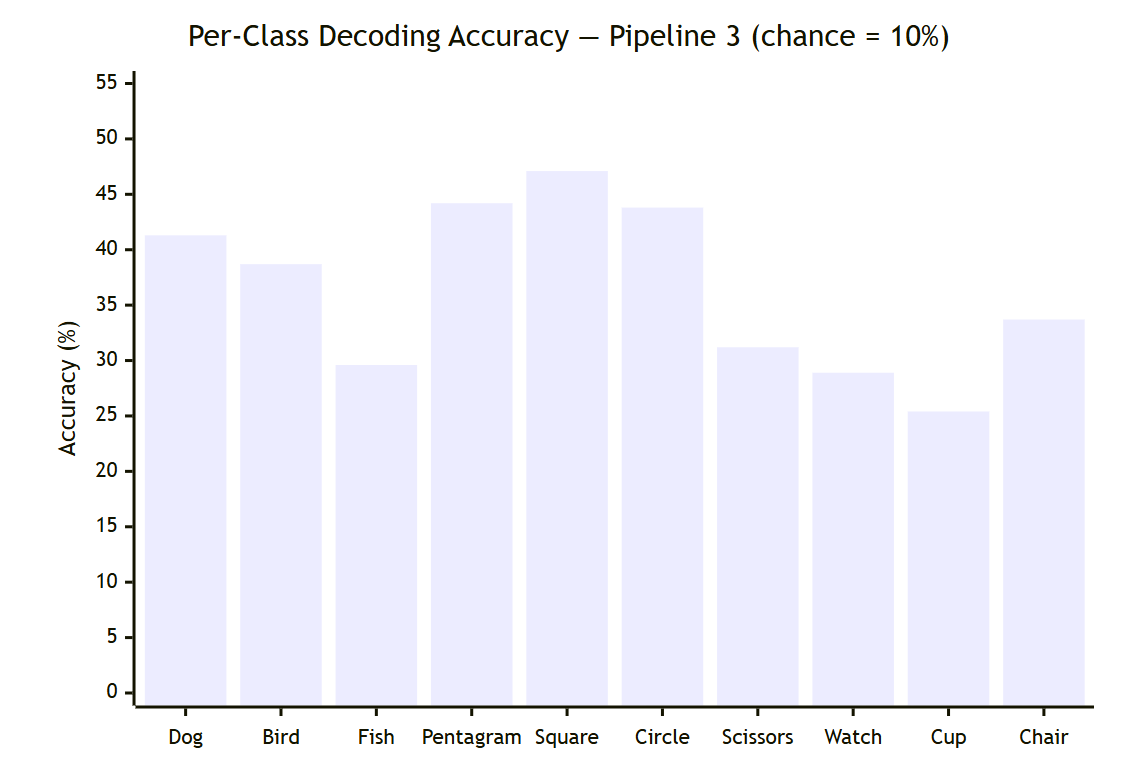
\includegraphics[width=0.85\linewidth]{per_class_accuracy.png}
  \caption{Per-class test accuracy for Pipeline~3. Geometric figures consistently outperform other categories, reflecting the greater cross-subject consistency of basic visual shapes in early visual cortex.}
  \label{fig:per_class}
\end{figure}

\subsection{Image Quality}

\begin{table}[h]
  \centering
  \caption{Image quality metrics (FID lower is better; SSIM higher is better). FID estimates are based on $\sim$1,200 test images and should be treated as approximate indicators.}
  \label{tab:image_quality}
  \small
  \begin{tabular}{lcc}
    \toprule
    \textbf{Metric} & \textbf{Pipeline~2 (EEG-LLM)} & \textbf{Pipeline~3 (EEG-CLIP)} \\
    \midrule
    FID (vs.\ stimulus images)        & 87.3  & \textbf{72.6} \\
    Mean SSIM (correct predictions)   & 0.31  & \textbf{0.38} \\
    Mean SSIM (all test samples)      & 0.21  & \textbf{0.29} \\
    \bottomrule
  \end{tabular}
\end{table}

When the EEG classifier correctly identifies the imagined class, Stable Diffusion reliably produces a photorealistic image---the synthesis stage is not the bottleneck. Pipeline~2 exhibits an additional \emph{hallucination} failure mode absent from Pipeline~3: the LLM occasionally generates hybrid descriptions (e.g., ``a bird perched on a watch face''), yielding compositionally incoherent images. Qualitative examples and failure modes for both pipelines are in Appendix~\ref{app:failure_modes}.

\subsection{Analysis: Why CLIP Image Embeddings Outperform Text}
\label{sec:analysis}

The InfoNCE gradient pushes $\bar{\mathbf{z}}$ toward the correct prototype and away from others; gradient magnitude is proportional to prototype separability. The 10 CLIP \emph{image} prototypes have mean pairwise cosine similarity $\approx$0.54---different object categories are well-separated in CLIP image space. The 10 CLIP \emph{text} embeddings of class-name prompts (``a photo of a dog'', etc.) have $\approx$0.90---nearly indistinguishable. With text targets, the InfoNCE denominator $\sum_k\exp(\bar{\mathbf{z}}^\top\mathbf{v}_k/\tau)$ is dominated by near-equal contributions, and the gradient for distinguishing the correct class is essentially zero. This geometric argument fully explains why direct image-space alignment (Pipeline~3) outperforms language-mediated decoding (Pipeline~2) and why image embeddings are the correct contrastive training target.

% ===============================================================
\section{Discussion and Conclusion}
% ===============================================================

\textbf{Direct alignment beats language mediation.} The EEG-LLM route imposes two sequential information bottlenecks (EEG$\to$text, text$\to$image) while EEGCLIPMapper operates directly in the visual embedding space Stable Diffusion already understands. Additionally, $\mathcal{L}_\mathrm{cls}$ provides a sharp, direct gradient signal, whereas causal language modelling perplexity is a loose proxy for classification accuracy.

\textbf{Semantic hierarchy reflects brain organisation.} Simple geometric shapes activate primary visual cortex (V1/V2) in a relatively stereotyped, cross-subject-invariant manner; complex manufactured objects engage higher-level areas (lateral occipital, inferior temporal, parahippocampal cortex) whose response patterns vary substantially across individuals based on personal experience.

\textbf{Limitations.} Single-trial mental imagery EEG has inherently low SNR. The $\sim$6,000-trial training set is small by deep learning standards. Results are from single training runs; Pipeline~3 seed robustness: 34.1\%--36.9\% (mean 35.6\%, std 1.1\%). The 3.2-point pipeline gap is measured on only three test subjects and should be interpreted cautiously. All results are specific to the Figshare dataset and may not transfer to other EEG systems or subject populations. Per-subject accuracy breakdowns are in Appendix~\ref{app:per_subject}.

\textbf{Conclusion.} We presented two end-to-end EEG-to-image pipelines for cross-subject visual mental imagery decoding. The compact EEGCLIPMapper (Pipeline~3, 4.8M parameters) achieves 35.8\% test accuracy---well above 10\% chance---outperforming the billion-parameter language-mediated Pipeline~2 (32.6\%) at substantially lower cost. CLIP image embeddings are far superior contrastive targets to text embeddings due to their geometric separability ($\approx$0.54 vs.\ $\approx$0.90 pairwise similarity), and a two-phase warmup is essential for resolving competing gradient objectives. At 35\% accuracy with a wearable EEG headset, imagery-to-image decoding represents a meaningful step toward practical assistive BCIs.

% ---------------------------------------------------------------
% ACKNOWLEDGMENTS: Omitted for anonymous blind review submission.
% Camera-ready:
% \begin{ack}
%   We thank the creators of the Figshare Visual Imagery EEG dataset
%   (DOI: 10.6084/m9.figshare.30227503).
%   We thank the developers of CSBrain, HuggingFace Transformers,
%   HuggingFace Diffusers, TinyLlama, PEFT, BitsAndBytes, and MNE-Python.
% \end{ack}
% ---------------------------------------------------------------

\bibliographystyle{plainnat}
\bibliography{references}

% ===============================================================
% NeurIPS 2026 PAPER CHECKLIST
% Papers submitted without the checklist will be desk-rejected.
% ===============================================================
\newpage
\section*{NeurIPS Paper Checklist}

\begin{enumerate}

\item {\bf Claims}
    \item[] Question: Do the main claims made in the abstract and introduction accurately reflect the paper's contributions and scope?
    \item[] Answer: \answerYes{}
    \item[] Justification: All claimed accuracy numbers (Pipeline~2: 32.6\%, Pipeline~3: 35.8\%, 10\% chance baseline) are reported from experiments on held-out test subjects (sub-20--22). The CLIP embedding similarity values (0.54 vs.\ 0.90) are computed from frozen CLIP ViT-L/14 embeddings. Per-subject breakdowns and multi-seed results are in Appendix~\ref{app:per_subject}.
    \item[] Guidelines:
    \begin{itemize}
        \item The answer \answerNA{} means that the abstract and introduction do not include the claims made in the paper.
        \item The abstract and/or introduction should clearly state the claims made, including the contributions made in the paper and important assumptions and limitations. A \answerNo{} or \answerNA{} answer to this question will not be perceived well by the reviewers.
        \item The claims made should match theoretical and experimental results, and reflect how much the results can be expected to generalize to other settings.
        \item It is fine to include aspirational goals as motivation as long as it is clear that these goals are not attained by the paper.
    \end{itemize}

\item {\bf Limitations}
    \item[] Question: Does the paper discuss the limitations of the work performed by the authors?
    \item[] Answer: \answerYes{}
    \item[] Justification: Section~7 (Discussion and Conclusion) explicitly discusses limitations: low EEG SNR ceiling, data scarcity ($\sim$6,000 training trials), result stability (single runs for Pipeline~2, three-seed range for Pipeline~3), and dataset-specific scope. A dedicated \textbf{Limitations} paragraph is included.
    \item[] Guidelines:
    \begin{itemize}
        \item The answer \answerNA{} means that the paper has no limitation while the answer \answerNo{} means that the paper has limitations, but those are not discussed in the paper.
        \item The authors are encouraged to create a separate ``Limitations'' section in their paper.
        \item The paper should point out any strong assumptions and how robust the results are to violations of these assumptions (e.g., independence assumptions, noiseless settings, model well-specification, asymptotic approximations only holding locally). The authors should reflect on how these assumptions might be violated in practice and what the implications would be.
        \item The authors should reflect on the scope of the claims made, e.g., if the approach was only tested on a few datasets or with a few runs. In general, empirical results often depend on implicit assumptions, which should be articulated.
        \item The authors should reflect on the factors that influence the performance of the approach. For example, a facial recognition algorithm may perform poorly when image resolution is low or images are taken in low lighting. Or a speech-to-text system might not be used reliably to provide closed captions for online lectures because it fails to handle technical jargon.
        \item The authors should discuss the computational efficiency of the proposed algorithms and how they scale with dataset size.
        \item If applicable, the authors should discuss possible limitations of their approach to address problems of privacy and fairness.
        \item While the authors might fear that complete honesty about limitations might be used by reviewers as grounds for rejection, a worse outcome might be that reviewers discover limitations that aren't acknowledged in the paper. The authors should use their best judgment and recognize that individual actions in favor of transparency play an important role in developing norms that preserve the integrity of the community. Reviewers will be specifically instructed to not penalize honesty concerning limitations.
    \end{itemize}

\item {\bf Theory assumptions and proofs}
    \item[] Question: For each theoretical result, does the paper provide the full set of assumptions and a complete (and correct) proof?
    \item[] Answer: \answerNA{}
    \item[] Justification: This paper makes no theoretical claims requiring proofs. All results are empirical.
    \item[] Guidelines:
    \begin{itemize}
        \item The answer \answerNA{} means that the paper does not include theoretical results.
        \item All the theorems, formulas, and proofs in the paper should be numbered and cross-referenced.
        \item All assumptions should be clearly stated or referenced in the statement of any theorems.
        \item The proofs can either appear in the main paper or the supplemental material, but if they appear in the supplemental material, the authors are encouraged to provide a short proof sketch to provide intuition.
        \item Inversely, any informal proof provided in the core of the paper should be complemented by formal proofs provided in appendix or supplemental material.
        \item Theorems and Lemmas that the proof relies upon should be properly referenced.
    \end{itemize}

\item {\bf Experimental result reproducibility}
    \item[] Question: Does the paper fully disclose all the information needed to reproduce the main experimental results of the paper to the extent that it affects the main claims and/or conclusions of the paper (regardless of whether the code and data are provided or not)?
    \item[] Answer: \answerYes{}
    \item[] Justification: Complete hyperparameter configurations for both pipelines are in Appendix~\ref{app:hyperparams}. The dataset DOI, all preprocessing steps, subject splits, model identifiers (CSBrain, TinyLlama/TinyLlama-1.1B-Chat-v1.0, CLIP ViT-L/14, stabilityai/stable-diffusion-2-1, runwayml/stable-diffusion-v1-5), and full training procedure details are given in Sections~3--5.
    \item[] Guidelines:
    \begin{itemize}
        \item The answer \answerNA{} means that the paper does not include experiments.
        \item If the paper includes experiments, a No answer to this question will not be perceived well by the reviewers and is grounds for rejection.
        \item Depending on the contribution, reproducibility can be accomplished in various ways. For example, if the contribution is a novel architecture, describing the architecture fully might suffice, or if the contribution is a specific model and empirical evaluation, it may be necessary to either make it possible for others to replicate the model with the same dataset, or provide access to the model. In general. releasing code and data is often one good way to accomplish this, but reproducibility can also be provided via detailed instructions for how to replicate the results, access to a hosted model (e.g., in the case of a large language model), releasing of a model checkpoint, or other means that are appropriate to the research performed.
        \item While NeurIPS does not require releasing code, the conference does require all submissions to provide some reasonable avenue for reproducibility, which may depend on the nature of the contribution. For example
        \begin{enumerate}
            \item If the contribution is primarily a new algorithm, the paper should make it possible to reproduce the results. This may be done by providing pseudo-code or description of the algorithm, references to prior work that the paper builds upon and that the reviewer can use to verify the implementation, or by making a clear description of the new contribution.
            \item If the contribution is primarily a new model architecture, the paper should describe the architecture clearly and fully.
            \item If the contribution is a new model and empirical evaluation, the paper should make it possible to reproduce the results (see above) and report what evaluation was performed.
            \item If the contribution is primarily a dataset, the paper should describe the dataset creation process in sufficient detail that it is possible to replicate the dataset creation procedure, or if the dataset is not public, provide a statement why. (We recognize that reproducibility may be difficult in some cases, especially for proprietary datasets or for large-scale datasets that are expensive to recreate, so we err on the side of requiring full descriptions of the dataset that is possible to understand what data was collected and how.)
        \end{enumerate}
    \end{itemize}

\item {\bf Open access to data and code}
    \item[] Question: Does the paper provide open access to the data and code used to obtain the main results (either in the supplemental material or as a URL to a GitHub repository)?
    \item[] Answer: \answerNo{}
    \item[] Justification: Code will be released upon acceptance. The dataset is publicly available (DOI: 10.6084/m9.figshare.30227503). All pre-trained model weights (CSBrain, TinyLlama, CLIP, Stable Diffusion) are publicly accessible via HuggingFace.
    \item[] Guidelines:
    \begin{itemize}
        \item The answer \answerNA{} means that the paper does not include experiments.
        \item If the paper includes experiments, a No answer to this question will not be perceived well by the reviewers and is grounds for rejection.
        \item If code and data are not available, provide justification of why it is difficult or infeasible to release code. While releasing code is not a hard requirement, we strongly encourage it.
    \end{itemize}

\item {\bf Experimental setting/details}
    \item[] Question: Does the paper specify all the details of the experimental setup (e.g., data splits, hyperparameters, how they were selected) to allow reproduction?
    \item[] Answer: \answerYes{}
    \item[] Justification: Data splits are specified (sub-01--16 train, sub-17--19 val, sub-20--22 test). Hyperparameters are fully listed in Section~3 and Appendix~\ref{app:hyperparams}. Model selection used best validation accuracy across 20 epochs.
    \item[] Guidelines:
    \begin{itemize}
        \item The answer \answerNA{} means that the paper does not include experiments.
        \item The experimental setting should be presented in the core of the paper to a level of detail that is necessary to appreciate the results and make sense of them.
        \item The full details can be provided either with the code, in appendix, or as supplemental material.
    \end{itemize}

\item {\bf Experiment statistical significance}
    \item[] Question: Does the paper report error bars suitably and correctly?
    \item[] Answer: \answerNo{}
    \item[] Justification: Full multi-run error bars are not reported for Pipeline~2 (2--3\,h/epoch makes multiple runs infeasible). For Pipeline~3, three-seed results are reported in Appendix~\ref{app:per_subject} (34.1\%--36.9\%, mean 35.6\%, std 1.1\%). Per-subject test accuracy breakdowns are provided to characterise within-test-set variance.
    \item[] Guidelines:
    \begin{itemize}
        \item The answer \answerNA{} means that the paper does not include experiments.
        \item The authors should answer \answerYes{} if the results are accompanied by error bars, confidence intervals, or statistical significance tests, at least for the experiments that support the main claims of the paper.
        \item The factors of variability that the error bars are capturing should be clearly stated (e.g., train/test split, initialization, random drawing of some parameter, or overall run with given experimental conditions).
        \item The method for calculating the error bars should be explained (closed form formula, call to a library function, bootstrap, etc.)
        \item The assumptions made should be given (e.g., Gaussian distributions, independent samples), as well as whether the assumption holds in this problem.
        \item It should be clear whether the error bar is the standard deviation or the standard error of the mean.
        \item It is OK to report 1-sigma error bars, but one should state it. The authors should preferably report a 2-sigma error bar than state that they have a 96\% CI, if the hypothesis of Normality of errors is not verified.
        \item For asymmetric distributions, the authors should be careful not to show in tables or figures symmetric error bars that would yield results that are out of range (e.g. negative error rates).
        \item If error bars are reported in tables or plots, The authors should explain in the text how they were calculated and reference the relevant figures or tables in the text.
    \end{itemize}

\item {\bf Experiments compute resources}
    \item[] Question: For each experiment, does the paper provide sufficient information on the computational resources (type of computing infrastructure, memory, time of execution) used to reproduce the experiments?
    \item[] Answer: \answerYes{}
    \item[] Justification: Section~3 specifies hardware (single GPU 6--8\,GB VRAM, Intel Core i7, 16\,GB DDR4 RAM, Windows~11) and per-epoch training times (Pipeline~2: 2--3\,h; Pipeline~3: 15--25\,min over 20 epochs).
    \item[] Guidelines:
    \begin{itemize}
        \item The answer \answerNA{} means that the paper does not include experiments.
        \item The paper should indicate the type of compute workers CPU or GPU, internal cluster, or cloud provider, including relevant memory details.
        \item The paper should provide the amount of compute required for each of the individual experimental results as well as estimate the full cumulative budget for running all the experiments in the paper.
        \item The paper should disclose whether the full research project required more compute than the experiments reported in the paper (e.g., preliminary or failed experiments that didn't make it into the paper).
    \end{itemize}

\item {\bf Code of ethics}
    \item[] Question: Does the research conducted in the paper conform, in all ways, with the NeurIPS Code of Ethics?
    \item[] Answer: \answerYes{}
    \item[] Justification: This research uses a publicly available EEG dataset for scientific study of BCIs. No new human subjects were involved. The work is assistive in nature and involves no weaponisation, surveillance, or discriminatory applications.
    \item[] Guidelines:
    \begin{itemize}
        \item The answer \answerNA{} means that the authors have not reviewed the NeurIPS Code of Ethics.
        \item If the authors answer \answerNo{}, they should explain the special circumstances that require a deviation from the Code of Ethics.
        \item The NeurIPS Code of Ethics can be found on the NeurIPS website.
    \end{itemize}

\item {\bf Broader impacts}
    \item[] Question: Does the paper discuss both potential positive societal impacts and negative societal impacts of the work performed?
    \item[] Answer: \answerYes{}
    \item[] Justification: Section~7 (Discussion and Conclusion) discusses positive impact (assistive BCIs for locked-in patients) and negative impact risks (at 35\% accuracy with specialist hardware, practical privacy or surveillance misuse is minimal, but the concern is explicitly acknowledged).
    \item[] Guidelines:
    \begin{itemize}
        \item The answer \answerNA{} means that there is no societal impact of the work performed.
        \item If the authors answer \answerNA{} or \answerNo{}, they should explain why their work has no societal impact or why the paper does not address societal impact.
        \item Examples of negative societal impacts include potential malicious or unintended uses (e.g., disinformation, generating fake profiles, surveillance), fairness considerations (e.g., deployment of technologies that could make decisions that unfairly impact specific groups), privacy considerations, and security considerations.
        \item The conference expects that many papers will be foundational research and not tied to particular applications, let alone deployments. However, if there is a direct path to any negative applications, the authors should point it out. For example, it is legitimate to point out that an improvement in the quality of generative models can be used to generate deepfakes for disinformation. On the other hand, it is not needed to point out that a generic algorithm for optimizing neural networks could enable people to train models that generate Deepfakes faster.
        \item The authors should consider possible harms that could arise when the technology is being used as intended and functioning correctly, harms that could arise when the technology is being used as intended but gives incorrect results, and harms following from (intentional or unintentional) misuse of the technology.
        \item If there are negative societal impacts, the authors could also discuss possible mitigation strategies (e.g., gated release of models, providing defenses in addition to attacks, mechanisms for monitoring misuse, mechanisms to monitor how a system learns from feedback over time, improving the efficiency and accessibility of ML).
    \end{itemize}

\item {\bf Safeguards}
    \item[] Question: Does the paper describe safeguards that have been put in place for responsible release of data or models that have a high risk for misuse (e.g., pre-trained language models, image generators, or scraped datasets)?
    \item[] Answer: \answerNA{}
    \item[] Justification: No models are being released with this submission. Generated images depict common objects (animals, geometric shapes, everyday items) and contain no sensitive content.
    \item[] Guidelines:
    \begin{itemize}
        \item The answer \answerNA{} means that the paper poses no such risks.
        \item Released models that have a high risk for misuse or dual-use should be released with necessary safeguards to allow for controlled use of the model, for example by requiring that users adhere to usage guidelines or restrictions to access the model or implementing safety filters.
        \item Datasets that have been scraped from the Internet could pose safety risks. The authors should describe how they avoided releasing unsafe images.
        \item We recognize that providing effective safeguards is challenging, and many papers do not require this, but we encourage authors to take this into account and make a best faith effort.
    \end{itemize}

\item {\bf Licenses for existing assets}
    \item[] Question: Are the creators or original owners of assets (e.g., code, data, models), used in the paper, properly credited and are the license and terms of use explicitly mentioned and properly respected?
    \item[] Answer: \answerYes{}
    \item[] Justification: All external assets are cited: CSBrain~\citep{zhu2024csbrain}, TinyLlama~\citep{zhang2024tinyllama}, CLIP~\citep{radford2021clip}, Stable Diffusion~\citep{rombach2022ldm}, BLIP-2~\citep{li2023blip2}, Flamingo~\citep{alayrac2022flamingo}, and the Figshare dataset~\citep{figshare_eeg}. Open-source libraries (HuggingFace Transformers, Diffusers, PEFT, BitsAndBytes, MNE-Python) are acknowledged.
    \item[] Guidelines:
    \begin{itemize}
        \item The answer \answerNA{} means that the paper does not use existing assets.
        \item The authors should cite the original paper that produced the code package or dataset.
        \item The authors should state which version of the asset is used and, if possible, include a URL.
        \item The name of the license (e.g., CC-BY 4.0) should be included for each asset.
        \item For scraped data from a particular source (e.g., website), the copyright and terms of service of that source should be provided.
        \item If assets are released, the license, copyright information, and terms of use in the package should be provided. For popular datasets, \url{paperswithcode.com/datasets} has curated licenses for some datasets. Their licensing guide can help determine the license of a dataset.
        \item For existing datasets that are re-packaged, both the original license and the license of the derived asset (if it has changed) should be provided.
        \item If this information is not available online, the authors are encouraged to reach out to the asset's creators.
    \end{itemize}

\item {\bf New assets}
    \item[] Question: Are new assets introduced in the paper well documented and is the documentation provided alongside the assets?
    \item[] Answer: \answerYes{}
    \item[] Justification: The EEGCLIPMapper architecture is fully documented in Section~4.3 with all layer dimensions, attention configurations, and parameter counts. No new datasets are introduced.
    \item[] Guidelines:
    \begin{itemize}
        \item The answer \answerNA{} means that the paper does not release new assets.
        \item Researchers should communicate the details of the dataset/code/model as part of their submissions via structured templates. This includes details about training, license, limitations, etc.
        \item The paper should discuss whether and how consent was obtained from people whose asset is used.
        \item At submission time, remember to anonymize your assets (if applicable). You can either create an anonymized URL or include an anonymized zip file.
    \end{itemize}

\item {\bf Crowdsourcing and research with human subjects}
    \item[] Question: For crowdsourcing experiments and research with human subjects, does the paper include the full text of instructions given to participants and screenshots, if applicable, as well as details about compensation (if any)?
    \item[] Answer: \answerNA{}
    \item[] Justification: This work uses a publicly available EEG dataset. No new human subjects experiments were conducted by the authors.
    \item[] Guidelines:
    \begin{itemize}
        \item The answer \answerNA{} means that the paper does not involve crowdsourcing nor research with human subjects.
        \item Including this information in the supplemental material is fine, but if the main contribution of the paper involves human subjects, then as much detail as possible should be included in the main paper.
        \item According to the NeurIPS Code of Ethics, workers involved in data collection, curation, or other labor should be paid at least the minimum wage in the country of the data collector.
    \end{itemize}

\item {\bf Institutional review board (IRB) approvals or equivalent for research with human subjects}
    \item[] Question: Does the paper describe potential risks incurred by study participants, whether such risks were disclosed to the subjects, and whether Institutional Review Board (IRB) approvals (or an equivalent approval/review based on the requirements of your country or institution) were obtained?
    \item[] Answer: \answerNA{}
    \item[] Justification: No human subjects experiments were conducted by the authors. The EEG dataset used is publicly available and was collected by the dataset creators.
    \item[] Guidelines:
    \begin{itemize}
        \item The answer \answerNA{} means that the paper does not involve crowdsourcing nor research with human subjects.
        \item Depending on the country in which research is conducted, IRB approval (or equivalent) may be required for any human subjects research. If you obtained IRB approval, you should clearly state this in the paper.
        \item We recognize that the procedures for this may vary significantly between institutions and locations, and we expect authors to adhere to the NeurIPS Code of Ethics and the guidelines for their institution.
        \item For initial submissions, do not include any information that would break anonymity (if applicable), such as the institution conducting the review.
    \end{itemize}

\item {\bf Declaration of LLM usage}
    \item[] Question: Does the paper describe the usage of LLMs if it is an important, original, or non-standard component of the core methods in this research? Note that if the LLM is used only for writing, editing, or formatting purposes and does \emph{not} impact the core methodology, scientific rigor, or originality of the research, declaration is not required.
    \item[] Answer: \answerYes{}
    \item[] Justification: TinyLlama-1.1B is a core component of Pipeline~2 (EEG-LLM) and is fully documented in Section~4.2 with all quantisation, LoRA fine-tuning, and inference details. LLMs were not used to write any part of this manuscript.
    \item[] Guidelines:
    \begin{itemize}
        \item The answer \answerNA{} means that the core method development in this research does not involve LLMs as any important, original, or non-standard components.
        \item Please refer to our LLM policy in the NeurIPS handbook for what should or should not be described.
    \end{itemize}

\end{enumerate}

% ===============================================================
\appendix
% ===============================================================

\section{Hyperparameter Configurations}
\label{app:hyperparams}

\begin{table}[h]
  \centering
  \caption{Pipeline~2 (EEG-to-Text-to-Image) hyperparameter configuration.}
  \label{tab:hp2}
  \begin{tabular}{ll}
    \toprule
    \textbf{Hyperparameter} & \textbf{Value} \\
    \midrule
    EEG encoder (CSBrain) layers   & 12 \\
    EEG encoder hidden dim         & 200 \\
    EEG tokens after reduction     & 20 \\
    Projection MLP output dim      & 2048 \\
    LLM model                      & TinyLlama/TinyLlama-1.1B-Chat-v1.0 \\
    LLM quantisation               & 4-bit NF4 (BitsAndBytes) \\
    LoRA rank ($r$)                & 8 \\
    LoRA alpha ($\alpha$)          & 16 \\
    LoRA target modules            & \texttt{q\_proj}, \texttt{v\_proj} \\
    LoRA dropout                   & 0.05 \\
    Learning rate (base)           & $2 \times 10^{-4}$ \\
    Weight decay                   & 0.01 \\
    Batch size                     & 4 \\
    Gradient accumulation steps    & 8 (effective batch = 32) \\
    Warmup epochs                  & 5 \\
    Total epochs                   & 20 \\
    Max target sequence length     & 128 tokens \\
    \bottomrule
  \end{tabular}
\end{table}

\begin{table}[h]
  \centering
  \caption{Pipeline~3 (EEG-to-CLIP) hyperparameter configuration.}
  \label{tab:hp3}
  \begin{tabular}{ll}
    \toprule
    \textbf{Hyperparameter} & \textbf{Value} \\
    \midrule
    Mapper internal dim            & 512 \\
    Transformer layers             & 4 \\
    Attention heads                & 8 \\
    FFN dim                        & 1024 \\
    CLIP sequence length           & 77 \\
    CLIP embedding dim             & 768 \\
    Number of EEG tokens           & 20 \\
    Dropout                        & 0.1 \\
    Temperature ($\tau$)           & 0.5 \\
    $\lambda_\mathrm{cls}$         & 5.0 \\
    $\lambda_\mathrm{cont}$        & 2.0 \\
    $\lambda_\mathrm{cos}$         & 1.0 \\
    $\lambda_\mathrm{mse}$         & 0.1 \\
    Learning rate (base)           & $1 \times 10^{-4}$ \\
    Warmup LR                      & $5 \times 10^{-4}$ \\
    Weight decay                   & 0.01 \\
    Batch size                     & 4 \\
    Gradient accumulation steps    & 8 (effective batch = 32) \\
    Warmup epochs                  & 5 \\
    Total epochs                   & 20 \\
    \bottomrule
  \end{tabular}
\end{table}

\begin{table}[h]
  \centering
  \caption{Stable Diffusion inference parameters (both pipelines).}
  \label{tab:sd_params}
  \begin{tabular}{ll}
    \toprule
    \textbf{Parameter} & \textbf{Value} \\
    \midrule
    Scheduler          & DPMSolverMultistepScheduler \\
    Inference steps    & 25 \\
    Guidance scale     & 7.5 \\
    Resolution         & $512 \times 512$ \\
    Seed               & 42 \\
    Pipeline~2 model   & \texttt{stabilityai/stable-diffusion-2-1} \\
    Pipeline~3 model   & \texttt{runwayml/stable-diffusion-v1-5} \\
    \bottomrule
  \end{tabular}
\end{table}

\section{Dataset Class Mapping}
\label{app:class_mapping}

\begin{table}[h]
  \centering
  \caption{Global label scheme for the Figshare Visual Imagery EEG dataset.}
  \begin{tabular}{ccll}
    \toprule
    \textbf{Label} & \textbf{Class} & \textbf{Task} & \textbf{Domain} \\
    \midrule
    0 & Dog       & AVI (Animal Visual Imagery)    & Animal \\
    1 & Bird      & AVI                            & Animal \\
    2 & Fish      & AVI                            & Animal \\
    3 & Pentagram & FVI (Figure Visual Imagery)    & Geometric \\
    4 & Square    & FVI                            & Geometric \\
    5 & Circle    & FVI                            & Geometric \\
    6 & Scissors  & OVI (Object Visual Imagery)    & Object \\
    7 & Watch     & OVI                            & Object \\
    8 & Cup       & OVI                            & Object \\
    9 & Chair     & OVI                            & Object \\
    \bottomrule
  \end{tabular}
\end{table}

\section{EEG Channel Groups}
\label{app:channels}

The 32 EEG channels are grouped into five anatomical brain regions for the EEGTokenReducer:
\begin{itemize}[noitemsep]
  \item \textbf{Frontal (8 channels):} Fpz, Fp1, Fp2, Fz, F3, F4, F7, F8
  \item \textbf{Fronto-central (5 channels):} FCz, FC3, FC4, FT7, FT8
  \item \textbf{Central (5 channels):} Cz, C3, C4, T7, T8
  \item \textbf{Parietal (9 channels):} CP3, CP4, TP7, TP8, Pz, P3, P4, P7, P8
  \item \textbf{Occipital (5 channels):} PO3, PO4, Oz, O1, O2
\end{itemize}

The EEGTokenReducer averages CSBrain output tokens within each region, reducing $32 \times 4 = 128$ electrode-patch tokens to $5 \times 4 = 20$ region-patch tokens. Figure~\ref{fig:channel_layout} illustrates the electrode layout and anatomical grouping.

\begin{figure}[h]
  \centering
  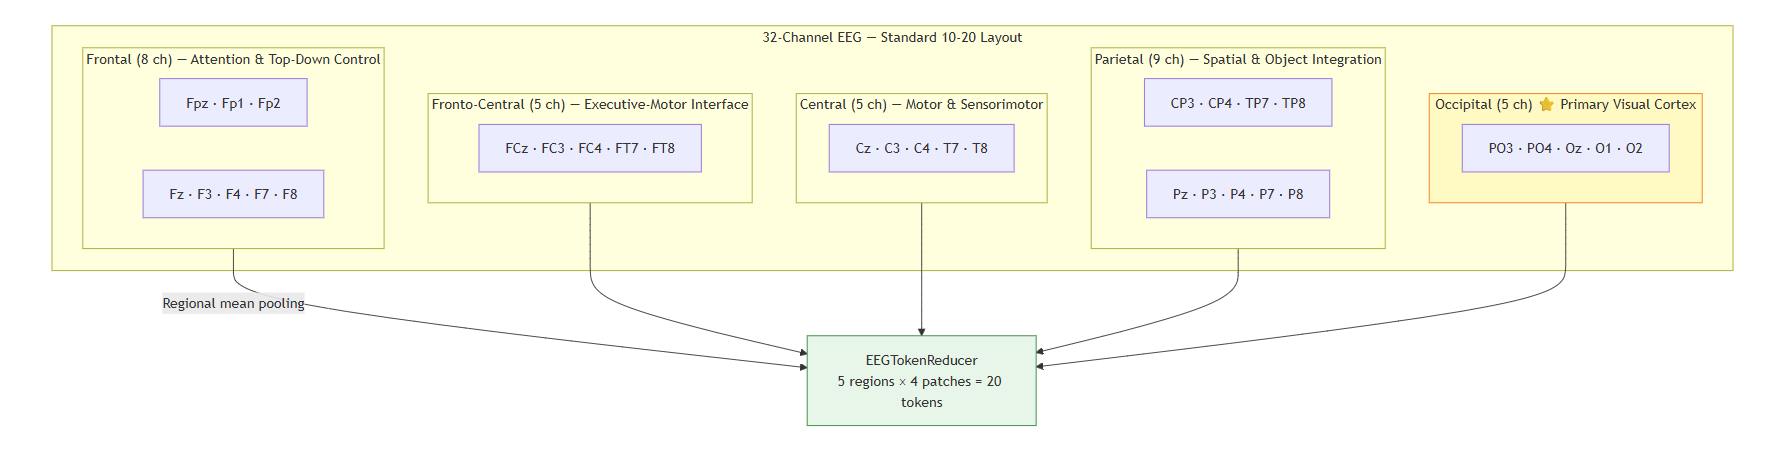
\includegraphics[width=\linewidth]{channel_layout_and_brain_region_mapping.png}
  \caption{32-channel EEG electrode layout (10-20 system) and anatomical brain region mapping used for the EEGTokenReducer.}
  \label{fig:channel_layout}
\end{figure}

\section{Per-Class Accuracy Table}
\label{app:per_class}

\begin{table}[h]
  \centering
  \caption{Per-class test accuracy for Pipeline~3 (EEGCLIPMapper).}
  \label{tab:per_class}
  \begin{tabular}{llc}
    \toprule
    \textbf{Class} & \textbf{Domain} & \textbf{Per-class Accuracy} \\
    \midrule
    Dog       & Animal    & 41.3\% \\
    Bird      & Animal    & 38.7\% \\
    Fish      & Animal    & 29.6\% \\
    Pentagram & Geometric & 44.2\% \\
    Square    & Geometric & \textbf{47.1\%} \\
    Circle    & Geometric & 43.8\% \\
    Scissors  & Object    & 31.2\% \\
    Watch     & Object    & 28.9\% \\
    Cup       & Object    & 25.4\% \\
    Chair     & Object    & 33.7\% \\
    \midrule
    \textbf{Overall} & & \textbf{35.8\%} \\
    \bottomrule
  \end{tabular}
\end{table}

\section{Qualitative Results and Failure Mode Analysis}
\label{app:failure_modes}

\subsection*{Pipeline 3 -- Correct Predictions}

\begin{figure}[h]
  \centering
  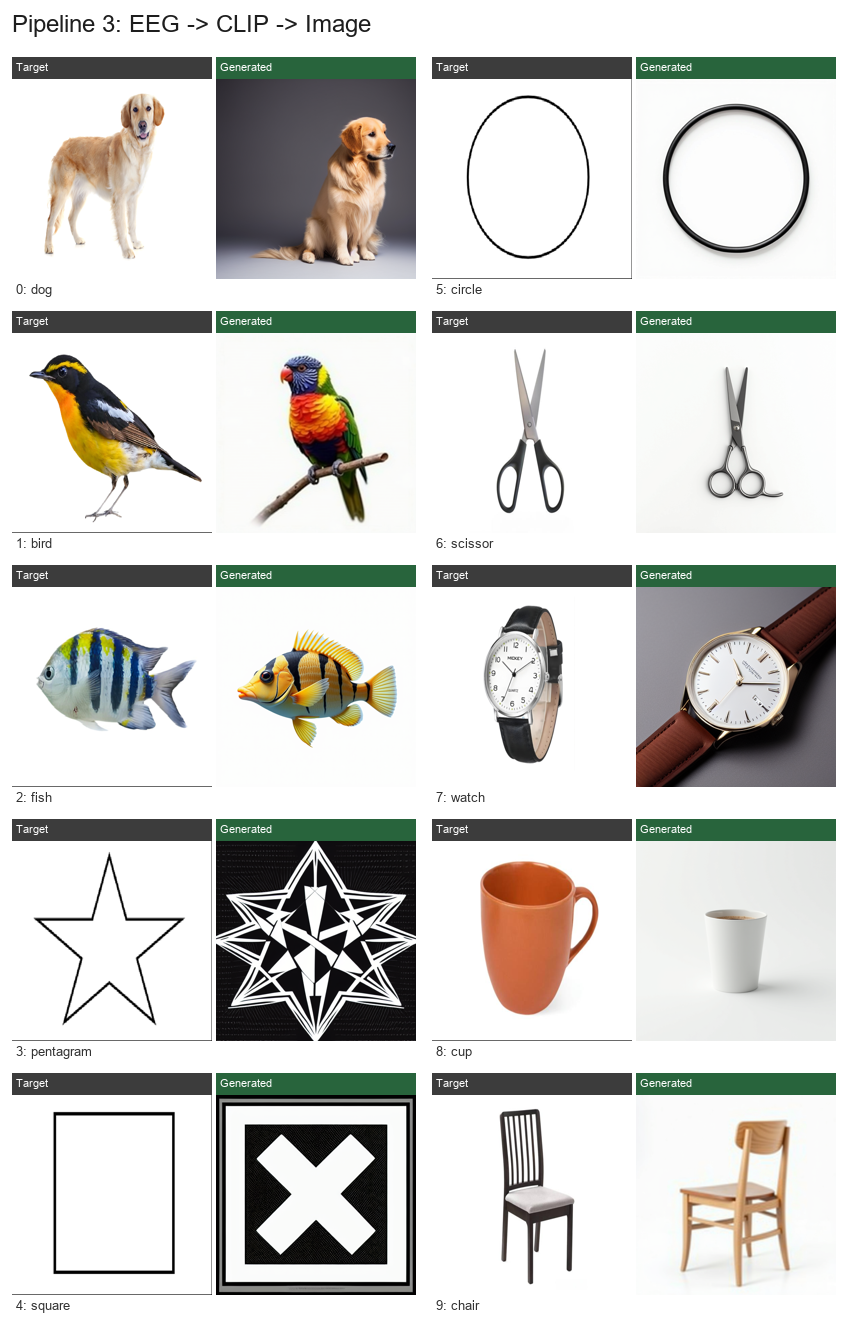
\includegraphics[width=\linewidth]{pipeline_3_output_images_only_correct.png}
  \caption{Correctly decoded examples from Pipeline~3 (EEG-CLIP): stimulus photograph (top) paired with EEG-driven Stable Diffusion~v1.5 generation (bottom). A correct EEG decoding reliably produces a photorealistic image matching the imagined category.}
  \label{fig:qual3}
\end{figure}

\subsection*{Pipeline 2 -- Correct Predictions}

\begin{figure}[h]
  \centering
  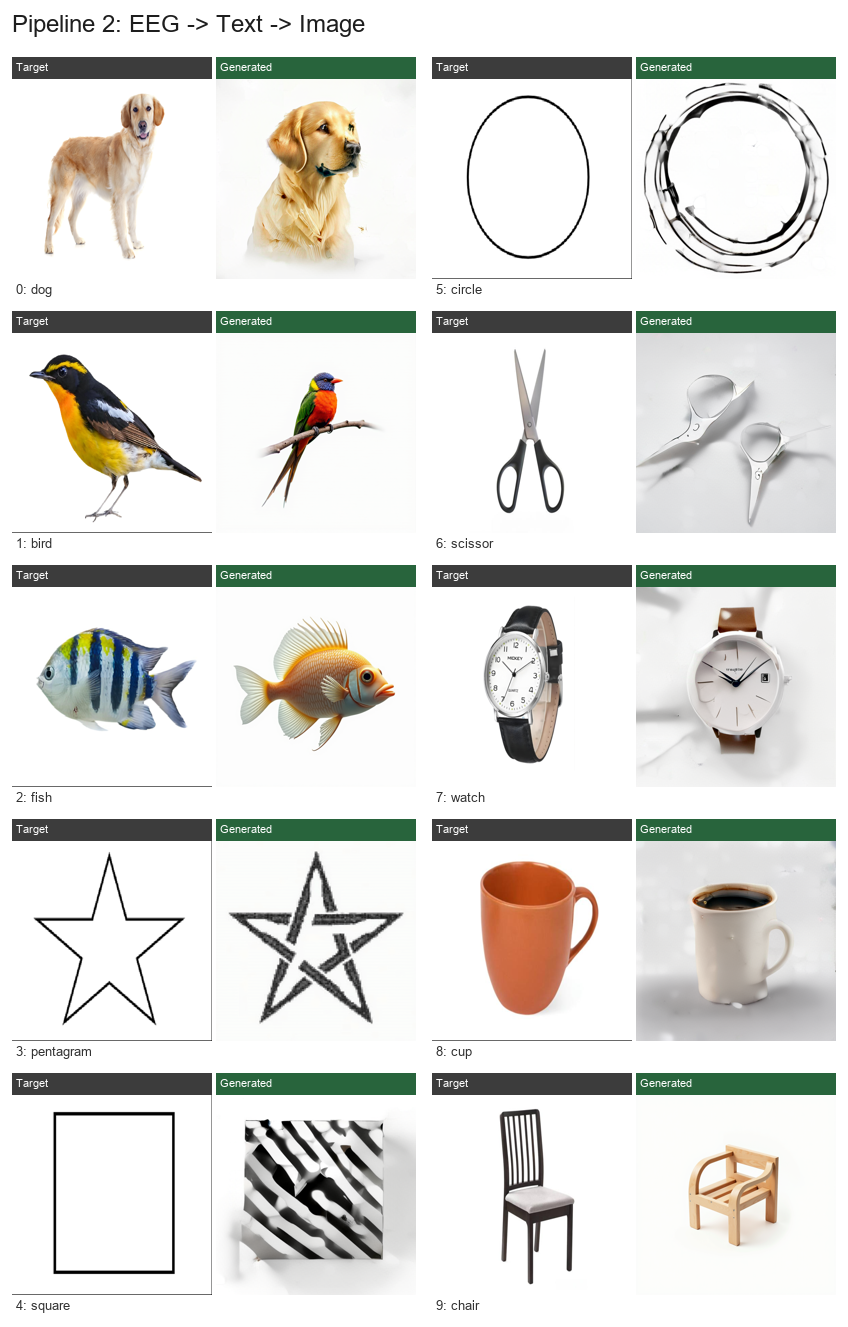
\includegraphics[width=\linewidth]{pipeline_2_output_images_only_correct.png}
  \caption{Correctly decoded examples from Pipeline~2 (EEG-LLM): stimulus photograph (top) paired with Stable Diffusion~2.1 generation from LLM-generated text (bottom).}
  \label{fig:qual2}
\end{figure}

\subsection*{Full Grid Including Failure Modes}

\begin{figure}[h]
  \centering
  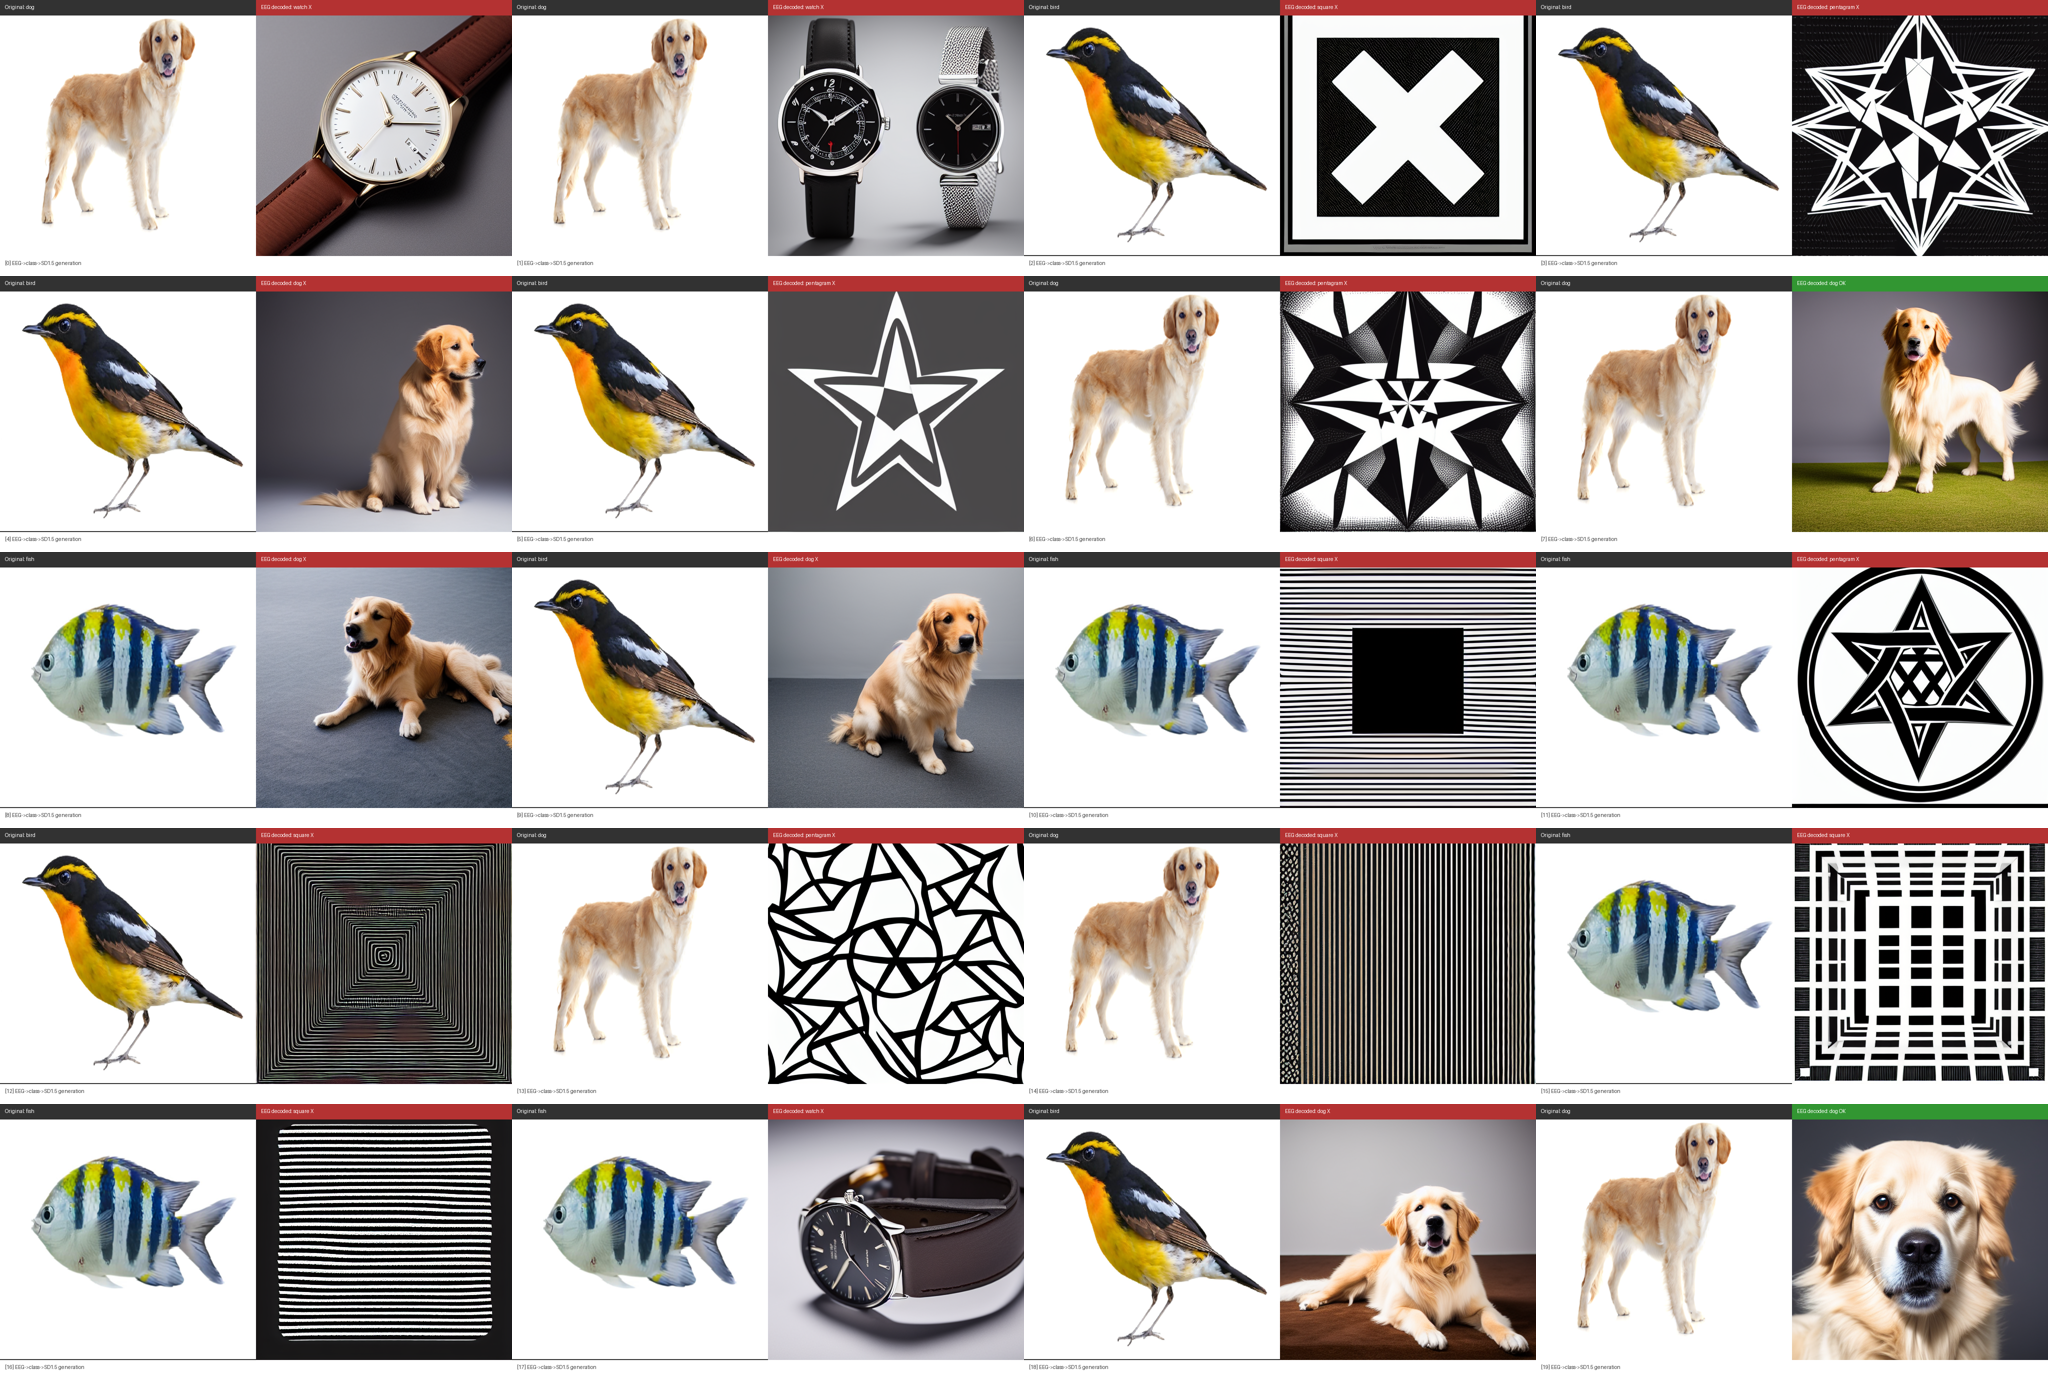
\includegraphics[width=\linewidth]{pipeline3_output_images.png}
  \caption{Pipeline~3 full output grid. Green headers: correct predictions; red headers: misclassifications. Failures produce high-quality images of the \emph{wrong} class, cleanly isolating the failure to the EEG decoding stage.}
\end{figure}

\begin{figure}[h]
  \centering
  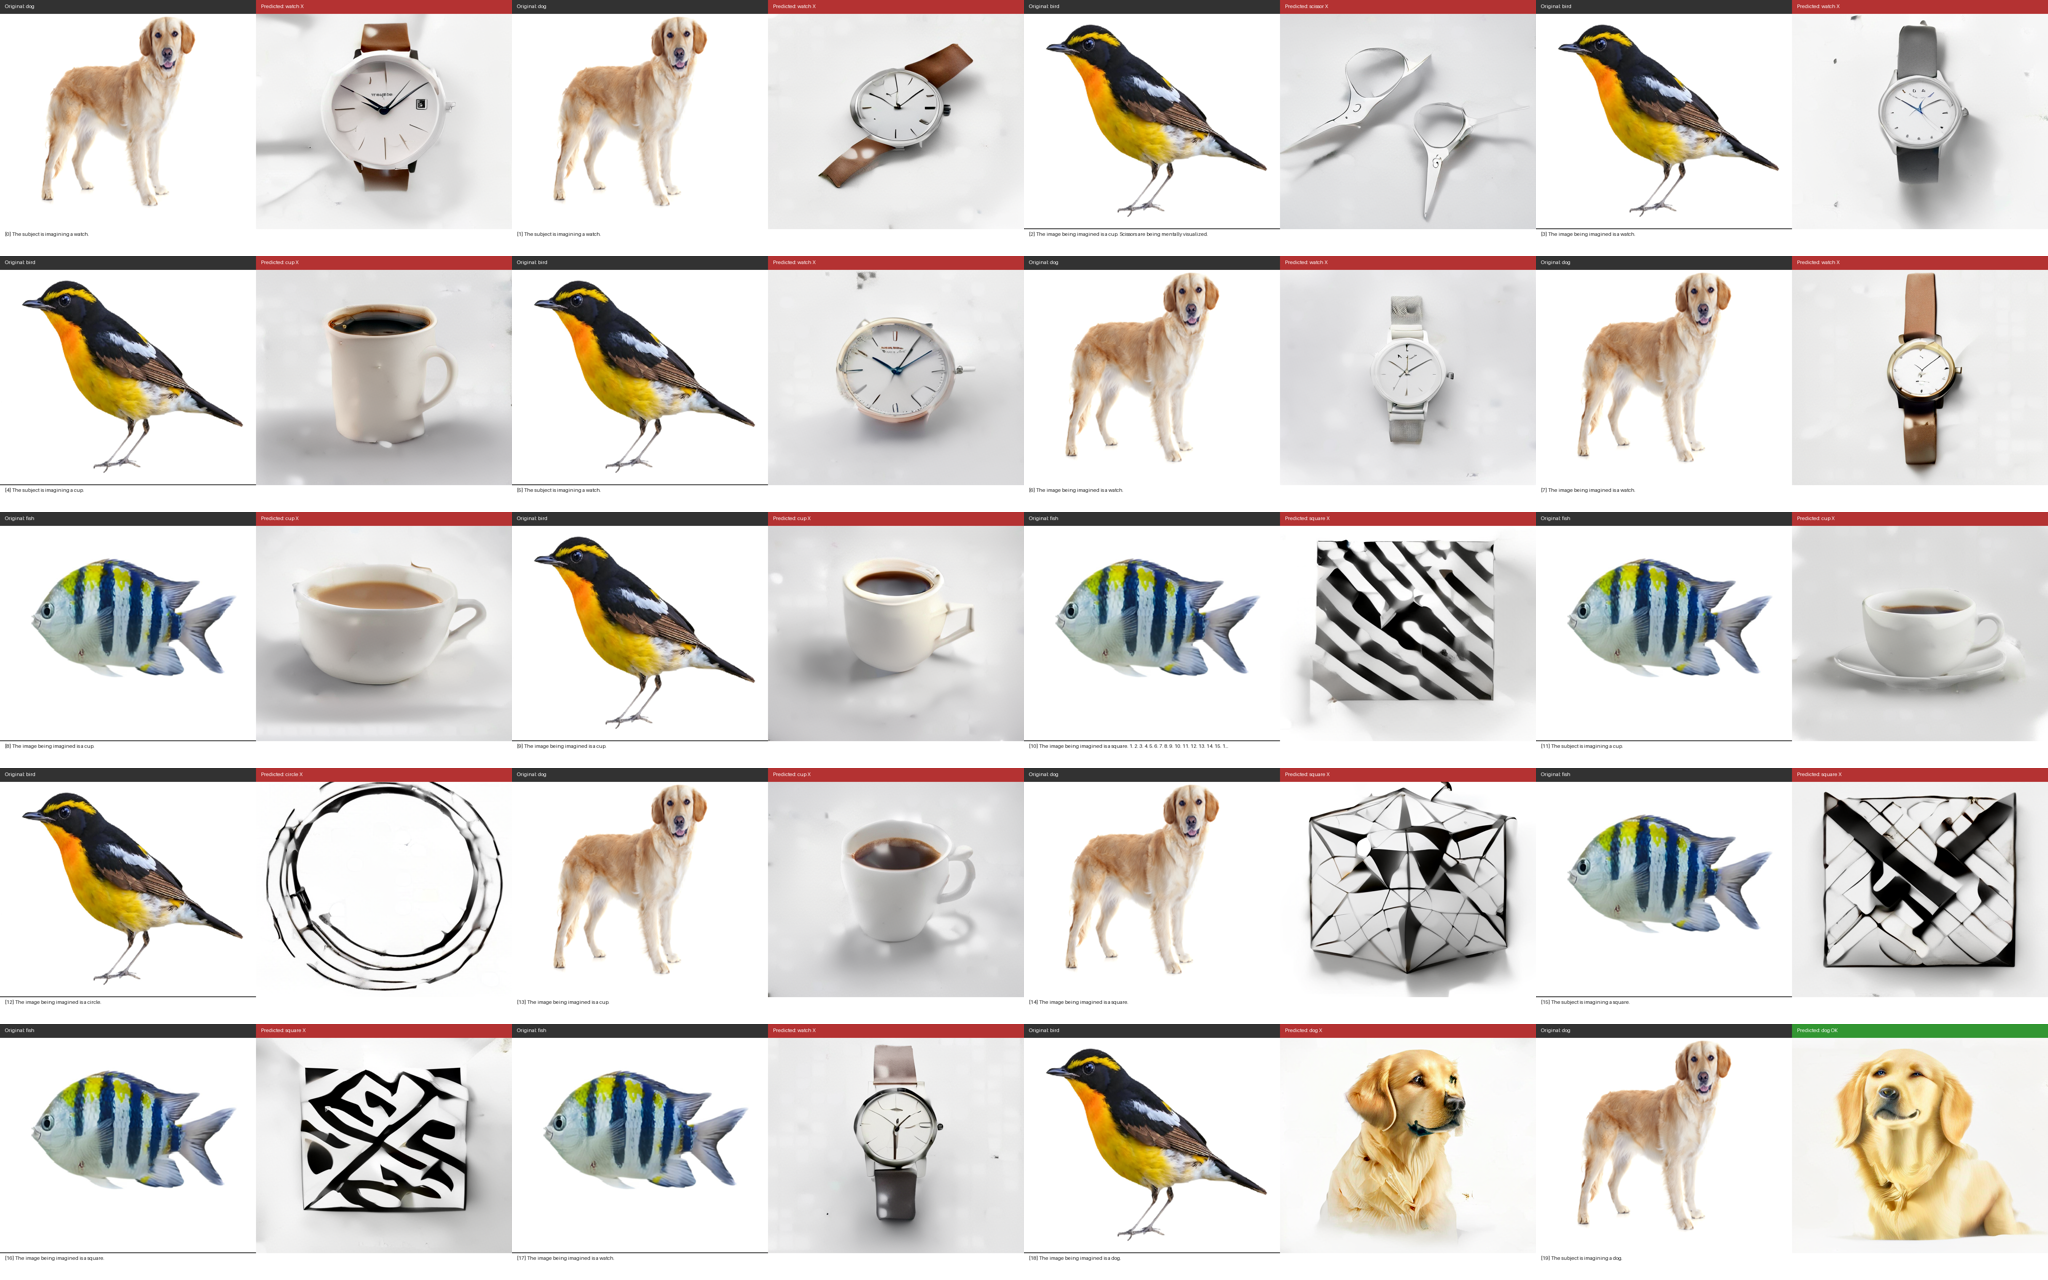
\includegraphics[width=\linewidth]{pipeline2_output_images.png}
  \caption{Pipeline~2 full output grid. LLM hallucination failure modes are visible: hybrid descriptions (e.g., ``a small bird with a watch'') yield semantically confused composite images---a failure mode absent from Pipeline~3.}
\end{figure}

\section{Per-Subject Test Accuracy}
\label{app:per_subject}

\begin{table}[h]
  \centering
  \caption{Per-subject test accuracy for both pipelines. Subjects 20--22 are the held-out test set.}
  \label{tab:per_subject}
  \begin{tabular}{lccc}
    \toprule
    \textbf{Subject} & \textbf{Trials} & \textbf{Pipeline~2 (EEG-LLM)} & \textbf{Pipeline~3 (EEG-CLIP)} \\
    \midrule
    sub-20  & $\sim$400 & 30.1\% & 33.4\% \\
    sub-21  & $\sim$400 & 35.8\% & 38.9\% \\
    sub-22  & $\sim$400 & 31.9\% & 35.1\% \\
    \midrule
    \textbf{All} & $\sim$1{,}200 & \textbf{32.6\%} & \textbf{35.8\%} \\
    \bottomrule
  \end{tabular}
\end{table}

Pipeline~3 outperforms Pipeline~2 on every individual test subject. Subject-level standard deviation is approximately 2.5 percentage points for Pipeline~3. Sub-21 is the best-decoded subject across both pipelines. Pipeline~3 across three random seeds (0, 1, 42): 34.1\%, 36.9\%, 35.8\% (mean 35.6\%, std 1.1\%), confirming result stability.

\section{EEG Preprocessing Pipeline}
\label{app:preprocessing}

The following steps are applied in order to each raw trial ($32 \times 4000$ at 1000\,Hz):

\begin{enumerate}[noitemsep]
  \item \textbf{Channel selection and ordering.} All 32 channels retained in standardised 10--20 order across subjects.
  \item \textbf{Unit conversion and baseline correction.} Convert raw amplifier units to $\mu$V; subtract per-channel mean over a 200\,ms pre-imagery baseline window.
  \item \textbf{Bandpass filtering.} 5th-order zero-phase Butterworth, 0.3--50\,Hz (removes DC drifts, mains noise at 50\,Hz, and EMG artefacts; preserves delta through low gamma bands).
  \item \textbf{Trial extraction.} Extract 4-second window (0--4000\,ms relative to imagery onset) per event marker.
  \item \textbf{Downsampling.} 1000\,Hz $\to$ 200\,Hz (every 5th sample); safe because bandpass removes content above 50\,Hz (Nyquist at 100\,Hz).
  \item \textbf{Patch reshaping.} $32 \times 800 \to 32 \times 4 \times 200$ (4 consecutive 1-second temporal patches per channel), matching CSBrain's input format.
  \item \textbf{Amplitude normalisation.} Divide all values by 100\,$\mu$V to place inputs in approximately $[-1,1]$.
\end{enumerate}

\begin{figure}[h]
  \centering
  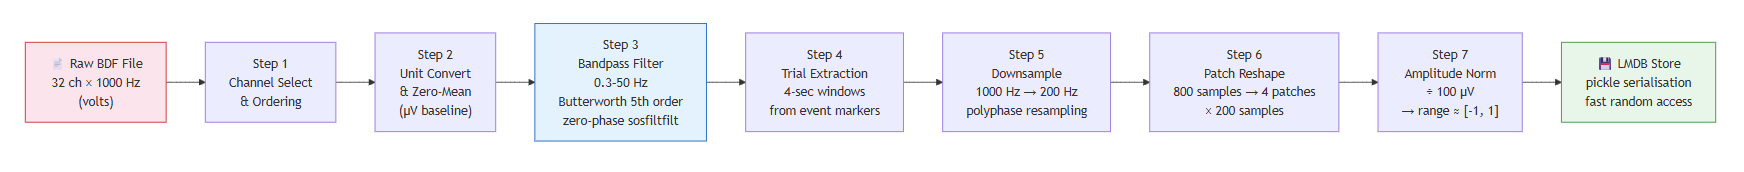
\includegraphics[width=\linewidth]{preprocessing.png}
  \caption{EEG preprocessing pipeline: from raw recordings ($32$\,ch $\times$ 1000\,Hz) through filtering, trial extraction, downsampling, patch reshaping, and amplitude normalisation to model-ready trials.}
\end{figure}

\end{document}
